\section{Calendar}

\subsection{Description of tasks}
A Work Breakdown Structure is performed and the following tasks are extracted:\\
\\
\begin{tabular}{|p{1cm}|p{4cm}|p{10cm}|}
\hline 
ID & Task & Description \\ 
\hline 
1 & Research about CFD and HT & Research about the evolution and current state of Computational Fluid Dynamics and Heat Transfer \\ 
\hline 
2 & Research about FVM & Research about the evolution and current state of the Finite Volumes Method \\ 
\hline 
3 & Research about conduction & Research about heat transfer by conduction between solids \\ 
\hline 
4 & Programming of a conduction code & Programming of a code about a problem in conduction between solids \\ 
\hline 
5 & Validation of the conduction code & Analysis of the validation of the code, as well as convergence study \\ 
\hline 
6 & Research about convection & Research about fluid dynamics and heat transfer in a laminar flow \\ 
\hline 
7 & Programming of a convection code & Programming of a code about a problem in fluid dynamics and heat transfer in a laminar flow \\ 
\hline 
8 & Validation of the convection code & Analysis of the validation of the code, as well as convergence study \\ 
\hline 
9 & Research about radiation & Research about heat transfer by radiation \\ 
\hline 
10 & Programming of a radiation code & Programming of a code about a problem in radiation \\ 
\hline 
11 & Validation of the radiation code & Analysis of the validation of the code, as well as convergence study \\ 
\hline 
12 & Programming of a combined code & Programming of a code about a problem combining conduction, convection and radiation \\ 
\hline 
13 & Validation of the combined code & Analysis of the validation of the code, as well as convergence study \\ 
\hline 
14 & Selection of a particular case & Selection of an industrial or aeronautical application in order to study it \\ 
\hline 
15 & Research about the particular case & Research about the particular application, evolution of its design, current methods used to design it \\ 
\hline 
16 & Programming of the particular case code & Programming of a code about the particular application \\ 
\hline 
17 & Validation of the particular case code & Analysis of the validation of the code, as well as convergence study \\ 
\hline 
18 & Optimization of the particular case code & Optimization of the different parameters of the selected application in order to obtain an optimum design \\ 
\hline 
\end{tabular}
\pagebreak

\subsection{Interdependency of tasks}
If not stated otherwise, all interdependencies between tasks are Begin-Finish.\\
\\
\begin{tabular}{|p{2cm}|p{4cm}|p{2cm}|p{2cm}|}
\hline 
ID & Task & Time & Dependency \\ 
\hline 
1 & Research about CFD & 20 h & - \\ 
\hline 
2 & Research about FVM & 20 h & 1 \\ 
\hline 
3 & Research about conduction & 10 h & 2 \\ 
\hline 
4 & Programming of a conduction code & 10 h & 3 \\ 
\hline 
5 & Validation of the conduction code & 5 h & 4 \\ 
\hline 
6 & Research about convection & 20 h & 5 \\ 
\hline 
7 & Programming of a convection code & 25 h & 6 \\ 
\hline 
8 & Validation of the convection code & 10 h & 7 \\ 
\hline 
9 & Research about radiation & 15 h & 8 \footnotemark \\ 
\hline 
10 & Programming of a radiation code & 15 h & 9 \\ 
\hline 
11 & Validation of the radiation code & 5 h & 10 \\ 
\hline 
12 & Programming of a combined code & 30 h & 11 \\ 
\hline 
13 & Validation of the combined code & 10 h & 12 \\ 
\hline 
14 & Selection of a particular case & 5 h & 13 \\ 
\hline 
15 & Research about the particular case & 15 h & 14 \\ 
\hline 
16 & Programming of the particular case code & 45 h & 15 \\ 
\hline 
17 & Validation of the particular case code & 10 h & 16 \\ 
\hline 
18 & Optimization of the particular case code & 30 h & 17 \\ 
\hline 
\end{tabular} 
\footnotetext{This task could start when task 2 finishes, but since the same person does all the tasks it is preferable to start task 9 when tasks 3, 4, 5, 6, 7 and 8 finish}

\subsection{Calendar of the project}
In order to develop the calendar, is has been supposed that the working schedule will be from Monday to Friday, working 4 hours a day.
\begin{landscape}
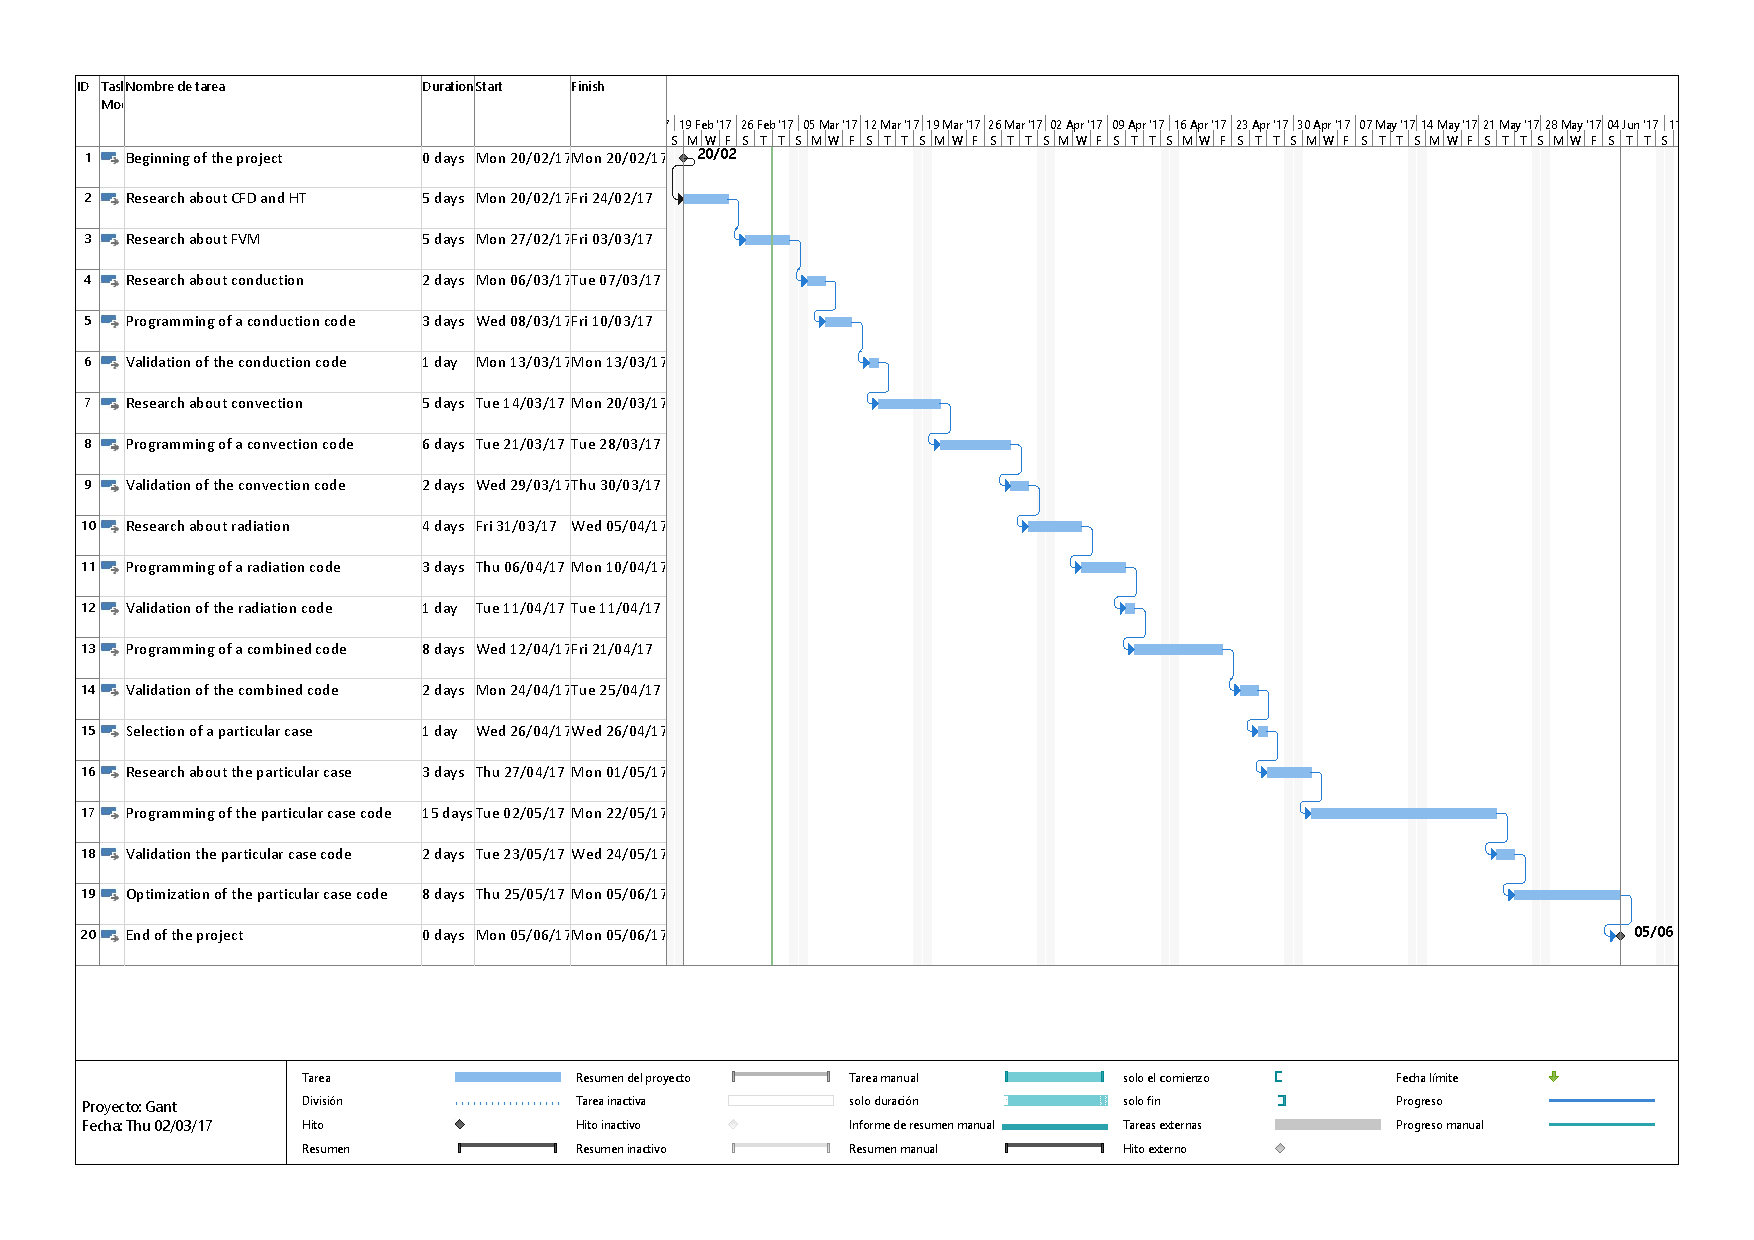
\includepdf[pages={1-}, landscape=true]{./Media/Gant.pdf}
\end{landscape}